\documentclass[10pt,letterpaper]{article}
\usepackage[margin=.85in]{geometry}
\usepackage[T1]{fontenc}\usepackage{lmodern,graphicx,booktabs,amsmath,xcolor,hyperref,xurl,caption,fancyhdr}
\hypersetup{colorlinks=true,urlcolor=teal,linkcolor=teal,pdftitle={Choose buildings for an energy review},pdfauthor={James Jean}}
\pagestyle{fancy}\fancyhf{}\fancyhead[L]{\small Building energy review / Study 28}\fancyhead[R]{\small Independent retrospective study}\fancyfoot[C]{\thepage}
\setlength{\headheight}{14pt}\setlength{\parindent}{0pt}\setlength{\parskip}{6pt}\captionsetup{font=small,labelfont=bf,hypcap=false}
\begin{document}
{\small\color{teal} BUILDING OPERATIONS / LIMITED REVIEW CAPACITY\par}
\vspace{7pt}{\LARGE\bfseries Choose buildings for an energy review\par}
\vspace{6pt}James Jean \hfill 30 October 2026
\section*{The decision}
An energy team with twenty review slots can focus on the largest energy users or on properties with high energy intensity relative to peers. These objectives produce different lists. This project supplies a reproducible comparison and a local scoring tool to help a reviewer see that choice before inspecting meter records, schedules or equipment.

In the screened 192-building 2023 review queue, the peer-relative and largest-consumption lists share \textbf{only 2 of 20 buildings}. Median floor area is \textbf{41,062.5 ft$^2$} in the peer list versus \textbf{707,905.0 ft$^2$} in the consumption list. The peer reference selected on development data is a simple property-type median; adding floor-area bins does not improve its development MAE.

\textbf{Practical recommendation.} Use a peer list when the question is unusual energy intensity for a property type, and a consumption list when the question is absolute annual energy use. Check source quality and the building's actual operation before acting. A flag does not establish waste, an equipment fault, noncompliance or achievable savings. No engineering review or realized benefit was measured.

\begin{center}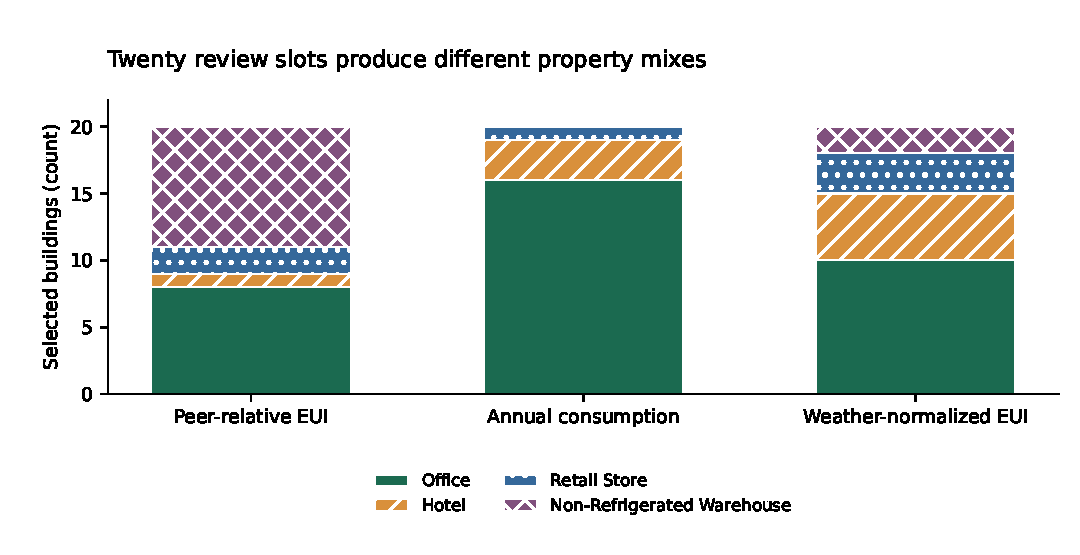
\includegraphics[width=.98\linewidth]{images/review_composition.pdf}\end{center}
\captionof{figure}{Equal review capacity, different property mixes. Each list contains twenty buildings, selected from the same 192 eligible current records. All property types remain visible. Capacities are hypothetical review scenarios, not measured staffing budgets.}

\textbf{Important limits.} Only 11 of the peer list's 20 selections have usable next-year follow-up; nine remain unavailable under the fixed rules. For forecasting next-year EUI, own prior-year EUI has held MAE 9.773 versus 22.958 for the peer reference. The peer comparison is structural context, not the winning forecasting model or an engineering efficiency certificate.

\newpage
\section*{1. What the source can establish}
NYC Department of Buildings disclosure dataset 5zyy-y8am [1] supplies the captured calendar years 2022--2024. The study population is four Portfolio Manager-calculated types: Office, Hotel, Retail Store and Non-Refrigerated Warehouse. It is a narrow subset of LL84 reporting, not all commercial properties or all buildings covered by the law. Current DOB guidance describes covered buildings over 25,000 gross square feet and additional categories [2]; older broad catalog descriptions may differ.

EUI is annual energy divided by floor area [3]. The target is the source's published \emph{weather-normalized site EUI}, in kBtu/ft$^2$/year. Its Portfolio Manager normalization is inherited, not independently refitted or validated here. Site energy used for the consumption list is the separately reported annual site-energy amount. A comparison of physical efficiency, weather models, emissions compliance or utility bills is outside the measured evidence.

The exact nineteen selected fields were captured as CSV and JSON. All 12,020 complete records match across formats as multisets, preserving duplicates: 228,380 selected cells. Forty-two row positions differed because source sort keys were tied; positional equality was corrected before model outcomes, without changing values. Independent Pandas/source projection checks passed 516,872 checks. Original selected responses and identity crosswalks stay private; public rows replace BIN/property identifiers with full SHA256 keys. Hashing public small-domain identifiers reduces direct exposure and does not guarantee anonymity.

\begin{center}\small\begin{tabular}{lrr}\toprule
Calendar year & Captured four-type rows & Eligible rows\\\midrule
2022 & 3764 & 2182 \\
2023 & 4032 & 951 \\
2024 & 4224 & 1106 \\
\bottomrule\end{tabular}\end{center}

The fixed screen retains 4,239 of 12,020 rows. It requires one valid standalone building, occupancy 80--100\%, 25,000--5,000,000 ft$^2$, consistent floor-area fields, positive bounded EUI and energy values, no reported estimated energy, and four selected meter alerts marked Ok. Site EUI and energy/area must agree within the declared rounding tolerance. These are declared screening assumptions, not proof of correct meters or physical efficiency. Missing and unknown tokens remain missing; repeated year/BIN keys and inconsistent property-to-BIN mappings are excluded in full.

All exclusions and overlapping reasons remain exported. In particular, 5,008 rows have estimated or unknown energy status and 1,689 lie on ambiguous year/BIN keys; these reason counts overlap and cannot be added as distinct buildings. Different eligible totals by year do not establish that physical building performance changed.

Current source records can be corrected or overwritten; the inspected NYC terms say older versions are not retained [4]. Before/after source-update metadata matched during capture. Initial per-response receipts were not saved before the first parser failure; the retained manifest explicitly labels captured-file write times and unknown original HTTP status. Raw hashes and fixed requests remain available. Original publication vintages and actual prior-year availability are unverified; this is an idealized retrospective input experiment.

\newpage
\section*{2. Entity separation and the peer reference}
Each BIN is assigned to a fixed bucket using the full SHA256 hash modulo five. Buckets 0--2 contribute 1,312 eligible 2022 training records. Bucket 3 supplies 145 validation pairs using 2022 features and 2023 EUI; bucket 4 supplies 119 held pairs using 2023 features and 2024 EUI. Paired records require a stable property type and next/current area ratio 0.8--1.25. No building hash crosses the three roles. Related source identities and ambiguous rows are screened before joining.

The peer model uses property type and prior-year floor area. Candidate zero is a pooled training median. Five candidates blend a type median with a type/area-bin median using weights $0,1/4,1/2,3/4,1$. Area bins have fixed boundaries 25,000, 50,000, 100,000, 250,000, 500,000, 1,000,000 and 5,000,001 ft$^2$. Groups need twenty training records: a sparse type falls back to the pool, and a sparse type/area bin falls back to its type reference. All medians and fallback counts are exported.

\[
\widehat{EUI}(x)=(1-\alpha)m_{\mathrm{type}}+\alpha m_{\mathrm{type,area}}.
\]

Choose among the six peer candidates by equal-building validation MAE in kBtu/ft$^2$/year. Exact ties prefer the lower candidate index. The own-prior-year EUI forecast is a fixed comparator, excluded from choosing a structural peer reference because it repeats the property's own level. Its comparison remains visible; the peer model is not claimed to be a better forecast. No R, GAM, boosting, embedding or optimization package was used; those broader historical ideas are not executed work.

\begin{center}\small\begin{tabular}{lrr}\toprule
Development comparator & MAE & RMSE\\\midrule
Pooled median & 26.914 & 36.586 \\
Type only & 25.650 & 35.125 \\
25\% size-bin weight & 25.735 & 35.193 \\
50\% size-bin weight & 25.827 & 35.299 \\
75\% size-bin weight & 25.976 & 35.443 \\
100\% size-bin weight & 26.135 & 35.626 \\
Own prior-year EUI & 22.041 & 151.373 \\
\bottomrule\end{tabular}\end{center}

The selected weight is zero: \textbf{type only}. Its exact validation MAE is $37193/1450$, or 25.650 kBtu/ft$^2$/year. Every attempted configuration remains reported. Size-bin detail increases overall validation MAE across this finite grid; no new grid was added. This is a boundary winner, not a global optimum or evidence that size never matters.

Prior-year persistence has lower validation MAE but much higher RMSE, reflecting large individual year-to-year changes. The reported source values and those failures were retained; there was no post-score trimming, threshold change or causal explanation. Twenty-one dependencies, including source, executable rules, independent checks, training medians and development exports, were hashed and committed at \texttt{6b789b6} before the separate held command. Source inputs and quality counts were unblinded; no analyst-blinding claim is made.

\newpage
\section*{3. Held prediction context}
On the 119 held annual pairs, type-only peer MAE is 22.958, compared with 26.547 for pooling and 9.773 for prior-year persistence. The type reference improves the pooled benchmark, while own history is the stronger forecast comparator. This result does not measure an engineer's ability to find faults or save energy.

\begin{center}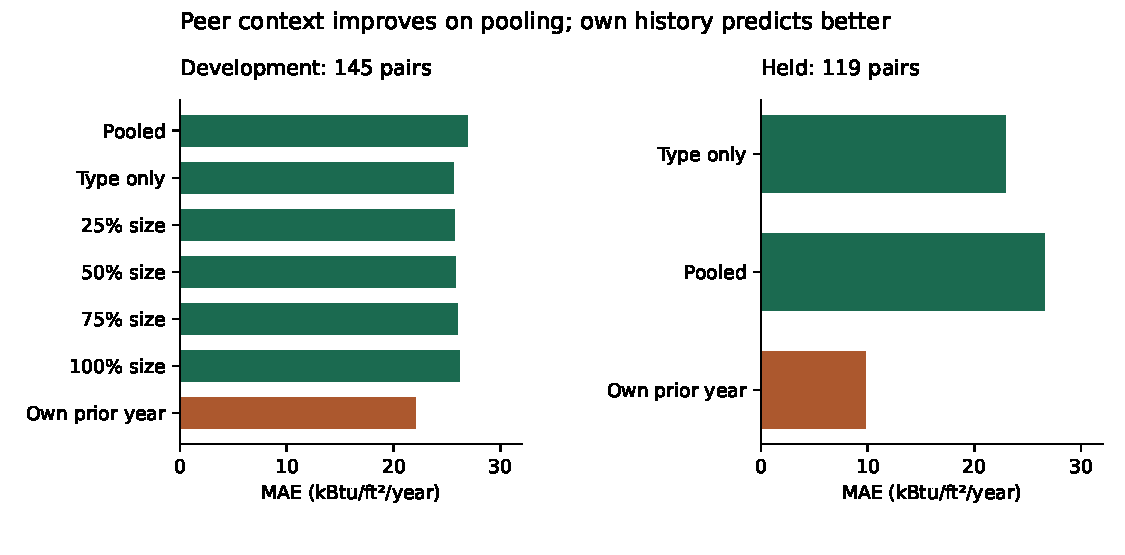
\includegraphics[width=.98\linewidth]{images/prediction_context.pdf}\end{center}
\captionof{figure}{Development and held MAE use the same units and zero-based horizontal scales. All six peer candidates and the fixed persistence comparator are visible in development. The held comparison uses the frozen selected/type reference, pooled reference and prior-year persistence; duplicate type references are not counted twice.}

\begin{center}\small\begin{tabular}{lrrrr}\toprule
Held comparator & MAE & MSE & RMSE & GFA-weighted MAE\\\midrule
Type only & 22.958 & 1006.881 & 31.731 & 20.479 \\
Pooled median & 26.547 & 1201.961 & 34.669 & 23.762 \\
Own prior-year EUI & 9.773 & 317.940 & 17.831 & 7.861 \\
\bottomrule\end{tabular}\end{center}

\begin{center}\small\begin{tabular}{lrrrr}\toprule
Property type & Pairs & Type MAE & Pooled MAE & Prior MAE\\\midrule
Office & 66 & 23.482 & 23.700 & 9.006 \\
Hotel & 16 & 16.700 & 32.112 & 10.844 \\
Retail Store & 13 & 30.862 & 31.031 & 15.423 \\
Non-Refrigerated Warehouse & 24 & 21.408 & 28.238 & 8.108 \\
\bottomrule\end{tabular}\end{center}

All property-type results are retained, including the small 13-pair retail stratum. No statistical significance, population-wide precision or prospective performance guarantee is claimed. MAE weights buildings equally; area-weighted MAE answers a different emphasis and is supplementary. MSE units are squared kBtu/ft$^2$/year; RMSE restores the original units.

\newpage
\section*{4. Equal-capacity review lists}
The review queue contains every eligible bucket-4 2023 record: 192 buildings. It is formed before requiring next-year follow-up. Three scores rank this same queue: weather-normalized EUI divided by the frozen peer reference; reported annual site energy; and weather-normalized EUI alone. Ties use ascending building hash. The 10\% illustration rounds up to twenty review slots.

\begin{center}\small\begin{tabular}{lrrrrr}\toprule
List & Selected & Follow-up & Missing & Median ft$^2$ & Median ratio\\\midrule
Peer-relative EUI & 20 & 11 & 9 & 41,062.5 & 1.943 \\
Annual consumption & 20 & 14 & 6 & 707,905.0 & 1.056 \\
Weather-normalized EUI & 20 & 12 & 8 & 65,674.5 & 1.922 \\
\bottomrule\end{tabular}\end{center}
{\small Median ratio uses only usable follow-up and divides 2024 EUI by the same frozen peer prediction from 2023 features. Missing values remain in the full selected denominator.}

\begin{center}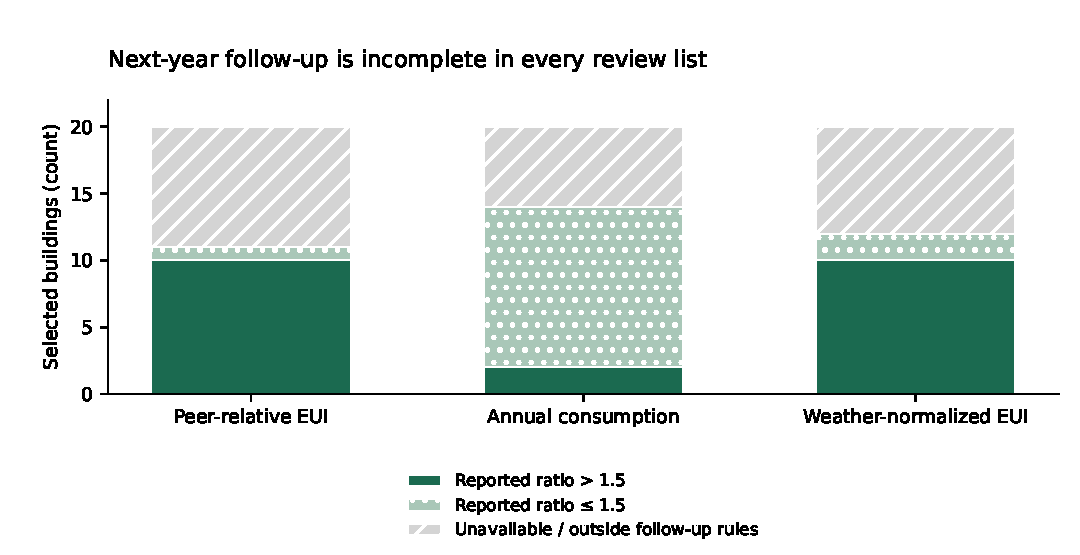
\includegraphics[width=.98\linewidth]{images/followup_coverage.pdf}\end{center}
\captionof{figure}{Observed and unavailable follow-up among all twenty selections. The fixed 1.5 band means later reported EUI exceeds 1.5 times the frozen peer reference. It is a descriptive relative-use threshold, not a calibrated fault/waste probability or a savings target. The other prespecified bands remain in the exports and table on the next page.}

The peer list contains ten known follow-up ratios above 1.5, one at or below 1.5 and nine unavailable. The consumption list contains two, twelve and six; the EUI list contains ten, two and eight. These lists select different properties, and follow-up is selective. Their conditional proportions do not establish relative engineering success or causal benefit.

Peer versus consumption has intersection 2 and union 38; peer versus EUI has intersection 13 and union 27; consumption versus EUI has intersection 4 and union 36. The peer list includes nine warehouses, compared with none in the largest-consumption list. This illustrates the operational tradeoff between relative intensity and absolute energy scale, not which buildings should receive a physical retrofit.

\newpage
\section*{5. Capacity and follow-up sensitivity}
All prespecified capacities are retained. The same ranking produces ten, twenty and thirty-nine selections at 5\%, 10\% and 20\% of the 192-building queue. These are hypothetical review capacities; the study does not measure actual staff throughput or review cost.

\begin{center}\small\begin{tabular}{llrrrr}\toprule
List & Capacity & Selected & Follow-up & Missing & Median ratio\\\midrule
Peer-relative EUI & 5\% & 10 & 4 & 6 & 2.362 \\
Peer-relative EUI & 10\% & 20 & 11 & 9 & 1.943 \\
Peer-relative EUI & 20\% & 39 & 23 & 16 & 1.724 \\
Annual consumption & 5\% & 10 & 5 & 5 & 1.260 \\
Annual consumption & 10\% & 20 & 14 & 6 & 1.056 \\
Annual consumption & 20\% & 39 & 26 & 13 & 1.140 \\
Weather-normalized EUI & 5\% & 10 & 5 & 5 & 1.645 \\
Weather-normalized EUI & 10\% & 20 & 12 & 8 & 1.922 \\
Weather-normalized EUI & 20\% & 39 & 22 & 17 & 1.608 \\
\bottomrule\end{tabular}\end{center}

\begin{center}\small\begin{tabular}{llrr}\toprule
10\% list & Ratio band & Above band & Usable denominator\\\midrule
Peer-relative EUI & 1.25 & 11 & 11 \\
Peer-relative EUI & 1.5 & 10 & 11 \\
Peer-relative EUI & 2 & 4 & 11 \\
Annual consumption & 1.25 & 5 & 14 \\
Annual consumption & 1.5 & 2 & 14 \\
Annual consumption & 2 & 0 & 14 \\
Weather-normalized EUI & 1.25 & 12 & 12 \\
Weather-normalized EUI & 1.5 & 10 & 12 \\
Weather-normalized EUI & 2 & 4 & 12 \\
\bottomrule\end{tabular}\end{center}

Nine missing peer-list outcomes comprise five invalid/ambiguous target records and four buildings absent from the captured four-type source rows. Missing does not mean low EUI or no energy problem. A building can leave this source population, change type, fail a quality rule or have an ambiguous record. Follow-up comparisons require the fixed stable-type/area rules and therefore do not represent all current selections.

\section*{6. Run a local review comparison}
{\raggedright \texttt{USAGE.md} describes the five-column input template and the distinction between the three lists. Use \texttt{src/score\_review.py} with the documented synthetic CSV, capacity 10 and a new output filename; the complete command is in \texttt{USAGE.md}. The three example records are invented interface fixtures, excluded from every research result. The tool scores a local, already quality-checked CSV, returns every rank and selected flag, rejects malformed/out-of-scope records and refuses to overwrite an existing output.\par}

Your portfolio's transfer performance is unvalidated. Format/range checks do not replace meter, identity, period or engineering checks. No external inference service or paid API is used for local scoring, and no owner names, contacts or addresses are needed.

\newpage
\section*{7. Evidence, limits and next action}
Independent source/projection checks passed 516,872 checks after the two captured formats matched all 228,380 selected cells. Independent decimal/rational arithmetic and SQLite identity/year/pair joins passed 302,146 development and 296,266 held checks, without importing production eligibility, fit or scoring helpers. Exact fractions govern medians, predictions, losses, weights, ranking and selection; decimal displays use twelve-place ties-to-even rounding. RMSE uses Decimal square roots at fifty-digit precision.

An isolated offline replay matched 103,262 CSV fields exactly and seven JSON documents, reran all 22 tests and the clearly synthetic CLI example, checked all 21 frozen dependencies and preserved the original exports. Three original figures have 31 source values, 248 SVG coordinate checks and nine hashes. These are finite checks, not universal correctness, physical validation or independent scientific peer review.

The source cohort is selective: four property types, single standalone buildings, high occupancy and strict reporting screens. Campus properties, ambiguous identities, unknown/estimated energy and missing or inconsistent measurements are excluded. The source's weather adjustment, owner-entered measurements, original release vintages and historical corrections are not independently established. Current revised rows are idealized past inputs; actual live decisions would require dated inputs and a new operational validation.

The initial source parser compared row positions despite tied sort keys; exact record-multiset comparison repaired that pre-analysis error. A fixed-decimal zero display test caught scientific notation, and an intermediate formatting edit introduced a type error before its bounded repair. Earlier files and failed outputs are retained privately; numerical model choices and the frozen selection were unchanged. The follow-up chart title was clarified to emphasize unavailable outcomes; values were unchanged. No held result was used to retune a model or eligibility bound.

\textbf{Next action.} Review source records and building operation for a small independently assessed sample from each list, including unflagged buildings and unavailable follow-up cases. Record genuine engineering findings and review effort before evaluating fault detection, actionable energy opportunities or savings. Retain the persistence forecast when the task is next-year prediction; choose the review-list objective explicitly. The present result supports a transparent comparison and working local tool, with engineering impact still unmeasured.

\textbf{Reproduce.} Install \texttt{requirements.txt}; run \texttt{python src/reproduce.py}, followed by the source, figure, manuscript and canonical-Git checks in the workflow. Replay uses the captured public projection offline. Full original-source reconciliation needs the separately retained private responses. Exact-head Linux checks, matching tested/merged trees and a verified remote annotated tag are required after local review; this paper's local evidence does not itself assert those later release gates passed. Formal-publication projects, including Azure optimization, remain excluded.

\section*{References}
{\small
[1] NYC DOB. LL84 annual disclosure 5zyy-y8am. \url{https://data.cityofnewyork.us/Environment/NYC-Building-Energy-and-Water-Data-Disclosure-for-/5zyy-y8am}. Captured 30 October 2026.\par
[2] NYC DOB. LL84 benchmarking law and covered buildings. \url{https://www.nyc.gov/site/buildings/codes/ll84-benchmarking-law.page}. Accessed 30 October 2026.\par
[3] EPA ENERGY STAR. What is energy use intensity? \url{https://www.energystar.gov/buildings/benchmark/understand-metrics/what-eui}. Accessed 30 October 2026.\par
[4] NYC Open Data. Terms of use. \url{https://data.cityofnewyork.us/stories/s/Terms-of-Use/k9k7-3cje}. Accessed 30 October 2026. No blanket CC0 or ownership claim is made.}
\end{document}
